
\documentclass{article}

% Page layout and margins
\usepackage[
	a4paper,
	bindingoffset=0.2in,
	left=1in,
	right=1in,
	top=1in,
	bottom=1in,
	footskip=.25in
]{geometry}

% Language
\usepackage[brazil]{babel}

% Math and symbols
\usepackage{amsmath, amssymb, mathtools}

% Algorithms
\usepackage[linesnumbered,ruled,vlined]{algorithm2e}

\SetKwIF{If}{ElseIf}{Else}{if}{:}{else if}{else}{end}
\SetKwFor{For}{for}{:}{end}
\SetKwRepeat{Do}{do}{while}
\SetKwProg{Function}{def}{:}{}

% Graphics and figures
\usepackage{graphicx}
\usepackage{subcaption}
\usepackage{caption}
\usepackage{float}
\usepackage{adjustbox}
\usepackage{tikz}

% Text formatting and layout
\usepackage{indentfirst}
\usepackage{fancyhdr}
\usepackage{quoting}
\usepackage{xcolor} % no need for [dvipsnames] unless you need extended colors

% URLs and hyperlinks
\usepackage{hyperref}
\usepackage{url}

% Code listings (optional, if you actually use it)
\usepackage{listings}

% Framed boxes (optional, if you use them)
\usepackage{tcolorbox}
\usepackage{mdframed}

% Citations
\usepackage{amsrefs} % or biblatex if preferred
\usepackage{cite}

\usepackage{setspace} % Para definir espaçamento entre linhas. (\onehalfspacing, \singlespacing, \doublespacing)
\usepackage{enumitem} % Para customizar listas (itemize, enumerate, etc.)

\definecolor{lightgray}{RGB}{240,240,240}

\newenvironment{blockquote}[1][lightgray]{\begin{mdframed}[
    leftline=true,
    topline=false,
    bottomline=false,
    rightline=false,
    linecolor=gray,
    linewidth=2pt,
    backgroundcolor=#1,
    skipabove=\baselineskip,
    skipbelow=\baselineskip,
    innerleftmargin=10pt,
    innerrightmargin=10pt,
    innertopmargin=5pt,
    innerbottommargin=5pt]
}
{\end{mdframed}}

% Counter for proof lines
\newcounter{proofline}

% Custom paired delimiters
\DeclarePairedDelimiter{\floor}{\lfloor}{\rfloor}
\DeclarePairedDelimiter{\ceil}{\lceil}{\rceil}
\DeclarePairedDelimiter{\abs}{\lvert}{\rvert}
\DeclarePairedDelimiter{\parens}{(}{)}
\DeclarePairedDelimiter{\curly}{\{}{\}}

% Box spacing tweaks
\setlength{\fboxsep}{0pt}
\setlength{\fboxrule}{1.4pt}

% Paragraph indent
\setlength{\parindent}{2em}

% Page style setup
\pagestyle{fancy}
\lhead{\footnotesize {\sc }}
\chead{}
\rhead{\footnotesize {\sc mac-ime-usp}}
\lfoot{}
\cfoot{}
\rfoot{\thepage}

\renewcommand{\headrulewidth}{0.5pt}
\renewcommand{\footrulewidth}{0.5pt}

\begin{document}

\begin{titlepage}

\begin{center}
	
	\begin{figure}[H]
		\centering
		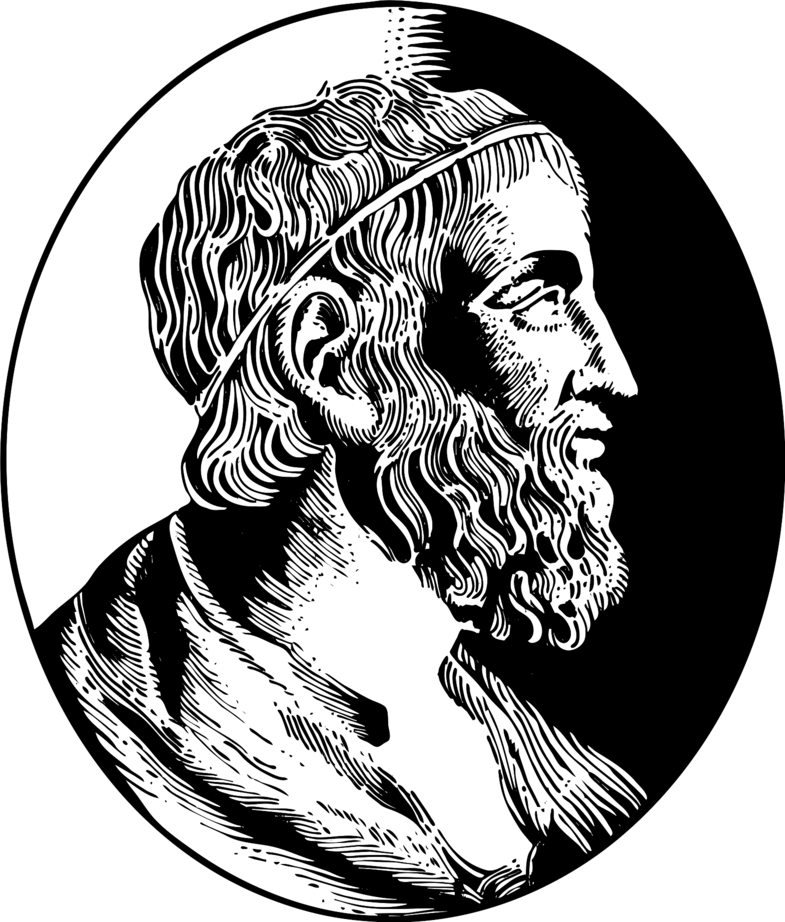
\includegraphics[width=0.3\textwidth]{logo-small.png} % Ajuste o caminho da imagem conforme necessário
	\end{figure}

	\vspace{2cm}

	{\Large \sc UNIVERSIDADE DE SÃO PAULO} \\
	{\Large \sc INSTITUTO DE MATEMÁTICA E ESTATÍSTICA} \\ [0.7cm]
	{\sc DEPARTAMENTO DE CIÊNCIA DA COMPUTAÇÃO} \\

	\vspace{2cm}

	\rule{\linewidth}{2pt}
	
	\vspace{0.2em} % Ajuste ao seu gosto
	{\Large \bfseries 
		O Problema da Visita de Polígonos \\
	}
	\vspace{0.2em} % Ajuste ao seu gosto
	
	\rule{\linewidth}{2pt} \\

\end{center}

\vspace{2.8cm}

\begin{center}
	{\large \bfseries Gabriel Freire Ushijima} \\
\end{center}

\vfill

% Data
\begin{center}
	\makeatletter
	{\large São Paulo, SP \\
	\@date}
	\makeatother
\end{center}

\end{titlepage}

\newpage

\section{Introdução}

Este relatório descreve a implementação e os resultados obtidos na resolução do problema da visita de polígonos, usando como base o paper de Mitchell \cite{mitchell2003} que descreve algoritmos para o caso sem e com restrições. Buscamos apresentar uma abordagem mais prática e detalhada para o problema, sem um foco tão grande na análise teórica.



\bibliography{referencias}

\end{document}
